\documentclass[a4paper,UTF8]{article}
\usepackage{ctex}
\usepackage[margin=1.25in]{geometry}
\usepackage{color}
\usepackage{graphicx}
\usepackage{amssymb}
\usepackage{amsmath}
\usepackage{amsthm}
\usepackage{enumerate}
\usepackage{bm}
\usepackage{hyperref}
\usepackage{epsfig}
\usepackage{tikz}
\usepackage{color}
\usepackage{mdframed}
\usepackage{lipsum}
\usepackage{graphicx}
\newmdtheoremenv{thm-box}{Theorem}
\newmdtheoremenv{prop-box}{Proposition}
\newmdtheoremenv{def-box}{定义}
\usetikzlibrary{shapes.geometric, arrows}

\usepackage{listings}
\usepackage{xcolor}
\lstset{
	numbers=left, 
	numberstyle= \tiny, 
	keywordstyle= \color{ blue!70},
	commentstyle= \color{red!50!green!50!blue!50}, 
	frame=shadowbox, % 阴影效果
	rulesepcolor= \color{ red!20!green!20!blue!20} ,
	escapeinside=``, % 英文分号中可写入中文
	xleftmargin=2em,xrightmargin=2em, aboveskip=1em,
	framexleftmargin=2em
} 

\usepackage{booktabs}

\setlength{\evensidemargin}{.25in}
\setlength{\textwidth}{6in}
\setlength{\topmargin}{-0.5in}
\setlength{\topmargin}{-0.5in}
% \setlength{\textheight}{9.5in}
%%%%%%%%%%%%%%%%%%此处用于设置页眉页脚%%%%%%%%%%%%%%%%%%
\usepackage{fancyhdr}                                
\usepackage{lastpage}                                           
\usepackage{layout}                                             
\footskip = 10pt 
\pagestyle{fancy}                    % 设置页眉                 
\lhead{2018年春季}                    
\chead{机器学习导论}                                                
% \rhead{第\thepage/\pageref{LastPage}页} 
\rhead{作业三}                                                                                               
\cfoot{\thepage}                                                
\renewcommand{\headrulewidth}{1pt}  			%页眉线宽,设为0可以去页眉线
\setlength{\skip\footins}{0.5cm}    			%脚注与正文的距离           
\renewcommand{\footrulewidth}{0pt}  			%页脚线宽,设为0可以去页脚线

\makeatletter 									%设置双线页眉                                        
\def\headrule{{\if@fancyplain\let\headrulewidth\plainheadrulewidth\fi%
\hrule\@height 1.0pt \@width\headwidth\vskip1pt	%上面线为1pt粗  
\hrule\@height 0.5pt\@width\headwidth  			%下面0.5pt粗            
\vskip-2\headrulewidth\vskip-1pt}      			%两条线的距离1pt        
 \vspace{6mm}}     								%双线与下面正文之间的垂直间距              
\makeatother  

%%%%%%%%%%%%%%%%%%%%%%%%%%%%%%%%%%%%%%%%%%%%%%
\numberwithin{equation}{section}
%\usepackage[thmmarks, amsmath, thref]{ntheorem}
\newtheorem{theorem}{Theorem}
\newtheorem*{definition}{Definition}
\newtheorem*{solution}{Solution}
\newtheorem*{prove}{Proof}
\newcommand{\indep}{\rotatebox[origin=c]{90}{$\models$}}

\usepackage{multirow}

%--

%--
\begin{document}
\title{机器学习导论\\
作业三}
\author{151220129, 吴政亿, nju\_wzy@smail.nju.edu.cn}
\maketitle



\section{[15pts] Decision Tree I}

\begin{enumerate}[ {(}1{)}]
	\item \textbf{[5pts]} 假设一个包含三个布尔属性${X, Y, Z}$的空间,并且目标函数是$f(x,y,z) = x\ \mathbf{XOR}\ z$,其中$\mathbf{XOR}$为异或运算符。令$H$为基于这三个属性的决策树,请问:目标函数$f$可实现吗?如果可实现,画出相应的决策树以证明;如果不可实现,请论证原因;
	
	\item \textbf{[10pts]} 现有如表~\ref{table:ranking}所示数据集:
	
	\begin{table}[!h]
		\centering
		\caption{样例表} \vspace{2mm}\label{table:ranking}
		\begin{tabular}{c c c|c}\hline
			$X$ & $Y$ & $Z$ & $f$ \\
			\hline
			$1$ & $0$  & $1$ &  $1$\\
			$1$ & $1$  & $0$ &  $0$\\
			$0$ & $0$  & $0$ &  $0$\\
			$0$ & $1$  & $1$ &  $1$\\
			$1$ & $0$  & $1$ &  $1$\\
			$0$ & $0$  & $1$ &  $0$\\
			$0$ & $1$  & $1$ &  $1$\\
			$1$ & $1$  & $1$ &  $0$\\
			\hline
		\end{tabular}
	\end{table}
	
	请画出由该数据集生成的决策树。划分属性时要求以信息增益 (information gain)为准则。当信息增益 (information gain)相同时,依据字母顺序选择属性即可。
\end{enumerate}
\begin{solution}
	此处用于写解答(中英文均可)
	\begin{enumerate}[ {(}1{)}]
		\item 
		\thispagestyle{empty}
		% 定义基本形状
		\tikzstyle{results}=[ellipse ,text centered,draw=black]
		\tikzstyle{decisions} =[rectangle, rounded corners,text centered, draw = black]
		% 箭头形式
		\tikzstyle{arrow} = [-,>=stealth]
		\begin{tikzpicture}[node distance=1cm]
		%定义具体形状和相关位置
		\node[decisions](rootnode){ X$=?$ };
		\node[decisions,below of=rootnode,yshift=-0.5cm,xshift=-2cm](z1){ Z$=?$ };
		\node[decisions,below of=rootnode,yshift=-0.5cm,xshift=2cm](z2){ Z$=?$ };
		\node[results,below of=z1,yshift=-0.5cm,xshift=-1cm](result1){0};
		\node[results,below of=z1,yshift=-0.5cm,xshift=1cm](result2){1};
		\node[results,below of=z1,yshift=-0.5cm,xshift=3cm](result3){0};
		\node[results,below of=z1,yshift=-0.5cm,xshift=5cm](result4){1};
		%连接形状
		\draw [arrow] (rootnode) -- node [left,font=\small] {1} (z1);
		\draw [arrow] (rootnode) -- node [right,font=\small] {0} (z2);
		\draw [arrow] (z1) -- node [right,font=\small] {1} (result1);
		\draw [arrow] (z1) -- node [left,font=\small] {0} (result2);
		\draw [arrow] (z2) -- node [right,font=\small] {1} (result3);
		\draw [arrow] (z2) -- node [left,font=\small] {0} (result4);
		\end{tikzpicture}
		
		\item
		首先计算根节点的信息熵:\\
		$$	Ent(D) = - \sum^{|\gamma|}_{k=1}{p_k\log_2{p_k}}
			=-(\frac{1}{2}\log_2{\frac{1}{2}}+\frac{1}{2}\log_2{\frac{1}{2}})=1$$
		然后计算每个属性的信息增益:\\
		\begin{equation*}
		\begin{aligned}
		&Gain(D,\mathbf{X}) &=& 0;\\
		&Gain(D,\mathbf{Y}) &=& 0;\\
		&Gain(D,\mathbf{Z}) &=& 1-\frac{6}{8}*(-\frac{4}{6}\log_2{\frac{4}{6}}+\frac{2}{6}\log_2{\frac{2}{6}})-\frac{2}{6}*0=0.311;
		\end{aligned}			
		\end{equation*}
		显然,$\mathbf{Z}$的信息增益最大,于是他被选为划分属性。\\
		当$\mathbf{Z}=0$时,$f$都等于1,当$\mathbf{Z}=1$时,可见应用$\mathbf{X}$与$\mathbf{Y}$的信息增益相同,因此根据字母顺序选择$\mathbf{X}$作为划分属性。
		
		\thispagestyle{empty}
		% 定义基本形状
		\tikzstyle{results}=[ellipse ,text centered,draw=black]
		\tikzstyle{decisions} =[rectangle, rounded corners,text centered, draw = black]
		% 箭头形式
		\tikzstyle{arrow} = [-,>=stealth]
		\begin{tikzpicture}[node distance=1cm]
		%定义具体形状和相关位置
		\node[decisions](rootnode){ $\mathbf{Z}=?$ };
		\node[decisions,below of=rootnode,yshift=-0.5cm,xshift=-2cm](x){ $\mathbf{X}=?$ };
		\node[decisions,below of=x,yshift=-0.5cm,xshift=-2cm](y1){ $\mathbf{Y}=?$ };
		\node[decisions,below of=x,yshift=-0.5cm,xshift=2cm](y2){ $\mathbf{Y}=?$ };
		\node[results,below of=rootnode,yshift=-0.5cm,xshift=2cm](result0){0};
		\node[results,below of=y1,yshift=-0.5cm,xshift=-1cm](result1){0};
		\node[results,below of=y1,yshift=-0.5cm,xshift=1cm](result2){1};
		\node[results,below of=y1,yshift=-0.5cm,xshift=3cm](result3){1};
		\node[results,below of=y1,yshift=-0.5cm,xshift=5cm](result4){0};
		%连接形状
		\draw [arrow] (rootnode) 	-- node [left,font=\small] 	{1} (x);
		\draw [arrow] (rootnode) 	-- node [right,font=\small] {0} (result0);
		\draw [arrow] (x) 			-- node [left,font=\small] 	{1} (y1);
		\draw [arrow] (x) 			-- node [right,font=\small] {0} (y2);
		\draw [arrow] (y1) 			-- node [left,font=\small] 	{1} (result1);
		\draw [arrow] (y1) 			-- node [right,font=\small] {0} (result2);
		\draw [arrow] (y2) 			-- node [left,font=\small] 	{1} (result3);
		\draw [arrow] (y2) 			-- node [right,font=\small] {0} (result4);
		\end{tikzpicture}
		
	\end{enumerate}
\end{solution}
\newpage



 \section{[20pts] Decision Tree II}
 考虑如下矩阵:
 $$
 \begin{bmatrix}
 4 & 6 & 9 & 1 & 7 & 5 \\
 1 & 6 & 5 & 2 & 3 & 4
 \end{bmatrix}^T
 $$

 该矩阵代表了$6$个样本数据,每个样本都包含$2$个特征$f_1$和$f_2$。这$6$个样本数据对应的标签如下:
 $$
 \begin{bmatrix}
 1 & 0 & 1 & 0 & 1 & 0
 \end{bmatrix}^T
 $$

 在这个问题中,我们要构造一个深度为$2$的树进行分类任务。

 \begin{enumerate}[ {(}1{)}]
 	\item \textbf{[5pts]} 请计算根结点 (root) 的熵值 (entropy);

 	\item \textbf{[10pts]} 请给出第一次划分的规则,例如$f_1 \geq 4, f_2 \geq 3$。对于第一次划分后产生的两个结点,请给出下一次划分的规则;

 	提示:可以直观判断,不必计算熵。

 	\item \textbf{[5pts]} 现在回到根结点 (root),并且假设我们是建树的新手。是否存在一种划分使得根结点 (root) 的信息增益 (information gain) 为$0$?
 \end{enumerate}

 \begin{solution}
 	此处用于写解答(中英文均可)
 	\begin{enumerate}[ {(}1{)}]
 		\item 首先计算根节点的信息熵:\\
 		$$	Ent(D) = - \sum^{|\gamma|}_{k=1}{p_k\log_2{p_k}}
 		=-(\frac{1}{2}\log_2{\frac{1}{2}}+\frac{1}{2}\log_2{\frac{1}{2}})=1$$
 		
 		\item 		\thispagestyle{empty}
 		% 定义基本形状
 		\tikzstyle{results}=[ellipse ,text centered,draw=black]
 		\tikzstyle{decisions} =[rectangle, rounded corners,text centered, draw = black]
 		% 箭头形式
 		\tikzstyle{arrow} = [-,>=stealth]
 		\begin{tikzpicture}[node distance=1cm]
 		%定义具体形状和相关位置
 		\node[decisions](rootnode){ $f_1=?$ };
 		\node[decisions,below of=rootnode,yshift=-0.5cm,xshift=-2cm](lchildnode){ $f_2=?$ };
 		\node[results,below of=rootnode,yshift=-0.5cm,xshift=2cm](result1){0};
 		\node[results,below of=lchildnode,yshift=-0.5cm,xshift=-1cm](result2){1};
 		\node[results,below of=lchildnode,yshift=-0.5cm,xshift=1cm](result3){0};
 		%连接形状
 		\draw [arrow] (rootnode) 	-- node [left,font=\small] 	{$f_1\leq6$} 	(lchildnode);
 		\draw [arrow] (rootnode) 	-- node [right,font=\small] {$f_1>6$} 		(result1);
 		\draw [arrow] (z1) 			-- node [left,font=\small] 	{$f_2\geq2$} 	(result2);
 		\draw [arrow] (z1) 			-- node [right,font=\small] {$f_2<2$} 		(result3);
 		\end{tikzpicture}
 		
 		\item 可以。我们根据$f_1 \leq 4$($f_2 \leq 2$,$f_2 \leq 4$也行)来划分,可以得到两个子集:\\
 		$D^1(f_1 \leq 4)$,$D^1(f_1 > 4)$。\\
 		计算他们各自的信息熵为:\\
 		\begin{equation*}
 		\begin{aligned}
		Ent(D^1)&=&-(\frac{1}{2}\log_2{\frac{1}{2}}+\frac{1}{2}\log_2{\frac{1}{2}})=1\\	Ent(D^2)&=&-(\frac{1}{2}\log_2{\frac{1}{2}}+\frac{1}{2}\log_2{\frac{1}{2}})=1
 		\end{aligned}			
 		\end{equation*}
 		信息增益为:
 		$$Gain(D,f_1) = Ent(D)-\sum_{v=1}^2{\frac{|D^v|}{|D|}Ent(D^v)}\\
 		=1-(\frac{2}{6}*1+\frac{4}{6}*1)=0$$
 	\end{enumerate}
 \end{solution}
\newpage

 \section{[25pts] Universal Approximator}
 已知函数$f:[-1, 1]^n \mapsto [-1, 1]$满足$\rho$-Lipschiz性质。 给定误差$\epsilon > 0$,请构造一个激活函数为\mbox{ sgn($\mathbf{x}$) }的神经网络$ \mathcal{N}:[-1,1]^n \mapsto [-1,1] $,使得对于任意的输入样本$ \mathbf{x} \in [-1,1]^n $,有$|f(\mathbf{x}) - \mathcal{N}(\mathbf{x})| \leq \epsilon$。\\
 (Lipschiz条件为:$ \forall \mathbf{x}, \mathbf{y} \in [-1,1]^n$,$ \exists \rho > 0$,$ \mbox{ s.t. } |f(\mathbf{x})-f(\mathbf{y})| \leq \rho \lVert \mathbf{x} - \mathbf{y} \rVert_2 $,其中\mbox{ sgn($\mathbf{x}$) }的定义参见《机器学习》第98页。)
 
  \begin{enumerate}[ {(}1{)}]
 	\item \textbf{[5pts]} 请画出构造的神经网络$\mathcal{N}$的示意图;
 	
 	\item \textbf{[10pts]} 请对构造的神经网络进行简要的说明(写清每一层的线性组合形式,也就是结点间的连接方式和对应的权重);
 	
 	\item \textbf{[10pts]} 证明自己构造的神经网络的拟合误差满足要求。
 \end{enumerate}


 \begin{solution}
	此处用于写解答(中英文均可)
	\begin{enumerate}[ {(}1{)}]
		\item 
	\end{enumerate}
 \end{solution}
\newpage

\section{[40pts] Neural Network in Practice}
通过《机器学习》课本第5章的学习,相信大家已经对神经网络有了初步的理解。深度神经网络在某些现实机器学习问题,如图像、自然语言处理等表现优异。本次作业旨在引导大家学习使用一种深度神经网络工具,快速搭建、训练深度神经网络,完成分类任务。

我们选取PyTorch为本次实验的深度神经网络工具,有了基础工具,我们就能如同搭积木一样构建深度神经网络。\href{http://pytorch.org/}{PyTorch}是Facebook开发的一种开源深度学习框架,有安装方便、文档齐全、构架方便、训练效率高等特点。本次作业的首要任务就是安装PyTorch。

目前PyTorch仅支持Linux和MacOS操作系统,所以Window用户需要装一个Linux虚拟机或者直接安装Linux系统。PyTorch安装很方便,只需要在其主页中的Get Start一栏选择对应的环境设置,便能够一键安装。有GPU的同学也可以尝试安装GPU版本的PyTorch。为保证此次作业的公平性,只要求使用CPU进行网络训练,当然有条件的同学也可以尝试使用GPU进行训练。在批改作业时,助教会提供Python 2.7、3.5、3.6三种环境进行实验验证。

我们选取CIFAR10作为本次作业的训练任务。\href{https://en.wikipedia.org/wiki/CIFAR-10}{CIFAR10}是一个经典的图片分类数据集,数据集中总共有60000张32$\times$32的彩色图片,总共有10类,每类6000张图片,其中50000张图片构成训练集,10000张图片构成测试集。PyTorch通过torchvision给用户提供了获取CIFAR10的方法,详细信息可见\href{http://pytorch.org/tutorials/beginner/blitz/cifar10_tutorial.html}{PyTorch的教程}。此外关于CIFAR10分类准确率排行可见此\href{http://rodrigob.github.io/are_we_there_yet/build/classification_datasets_results.html}{链接}。

下面我们将尝试使用PyTorch来解决实际问题:

\begin{enumerate}[(1)]
	\item \textbf{[15pts]} 首先我们跟随PyTorch的教程,用一个简单的卷积神经网络(Convolutional Neural Network, CNN),完成CIFAR10上的分类任务,具体要求如下:
	
	\begin{itemize}
		\item \textbf{[7pts]} 在代码实现之前,大家可能需要对CNN网络进行一定的了解,请大家自行查阅资料(PyTorch的教程中也有部分介绍CNN网络),并在实验报告中给出对CNN的见解:主要回答什么是卷积层,什么是Pooling层,以及两者的作用分别是什么;
		\item \textbf{[8pts]} 接下来就是具体的代码实现和训练。教程会手把手教你完成一次训练过程,其中使用SGD作为优化方法,请同学们自行调整epoch的大小和学习率,完成此次训练。另外,请在实验报告中给出必要的参数设置,以及训练结果如最终的loss、在测试集上的准确率等;
	\end{itemize}
	\item \textbf{[20pts]} 显然,这样一个简单的网络在CIFAR10上并不能取得令人满意的结果,我们需要选取一个更为复杂的网络来提升训练效果。在此小题中,我们选取了CIFAR10准确率排行榜上排名第二的结构,具体参见\href{https://arxiv.org/pdf/1412.6806.pdf}{论文链接}。为了方便大家实现,我们直接给出了网络结构如图\ref{network_structure}所示。请大家搭建完成此网络结构,并选择Adam为优化器,自行调整相关参数完成训练和预测,实验结果报告内容同第(1)小题;
	\begin{figure}[!h]
		\centering   
		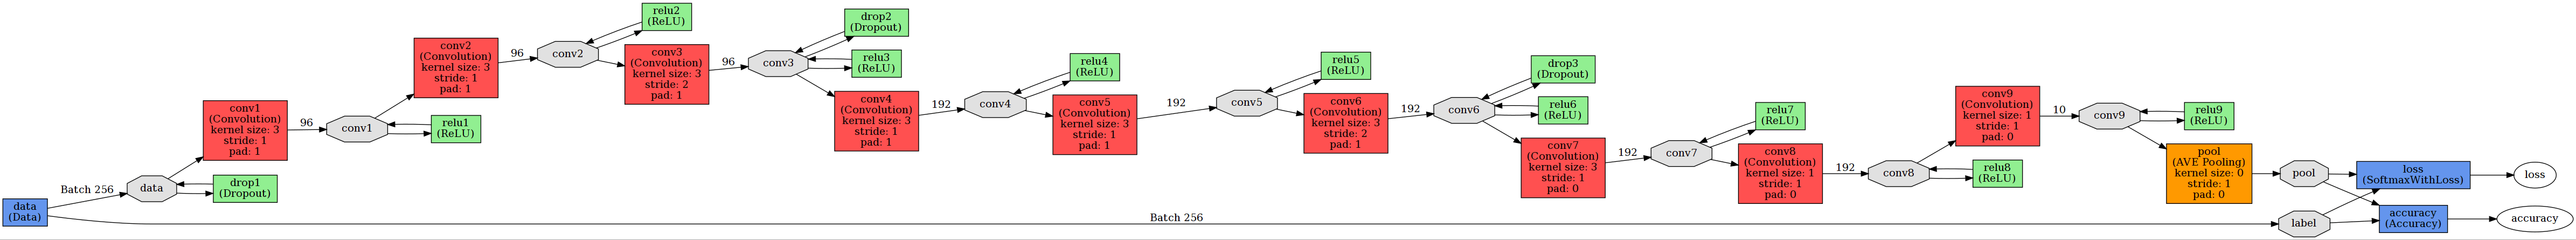
\includegraphics[width=0.99\textwidth, height=0.15\textwidth]{nn_structure.png}  
		\caption{待实现网络结构} 
		\label{network_structure}
	\end{figure}
	\item \textbf{[5pts]} 通过上一题实验我们可以发现,即使使用现成的网络结构也不一定能达到与其相同的训练效果。请大家分析其中的原因,并谈谈本次实验的感想,以及对深度学习调参的体会。
\end{enumerate}

\noindent{\textbf{实验报告.}}
\begin{enumerate}[(1)]
	\item 
	\subsection{卷积神经网络简介}
	卷积神经网络(Convolutional Neural Network, CNN)是一种前馈神经网络,它的人工神经元可以响应一部分覆盖范围内的周围单元,对于大型图像处理有出色表现。卷积神经网络与普通神经网络的区别在于,卷积神经网络包含了一个由卷积层和子采样层构成的特征抽取器。在卷积神经网络的卷积层中,一个神经元只与部分邻层神经元连接。在CNN的一个卷积层中,通常包含若干个特征平面(featureMap),每个特征平面由一些矩形排列的的神经元组成,同一特征平面的神经元共享权值,这里共享的权值就是卷积核。卷积核一般以随机小数矩阵的形式初始化,在网络的训练过程中卷积核将学习得到合理的权值。共享权值(卷积核)带来的直接好处是减少网络各层之间的连接,同时又降低了过拟合的风险。子采样也叫做池化(pooling),通常有均值子采样(mean pooling)和最大值子采样(max pooling)两种形式。子采样可以看作一种特殊的卷积过程。卷积和子采样大大简化了模型复杂度,减少了模型的参数。
	\subsection{定义介绍}
	卷积神经网络通常包含以下几种层:\\
	\begin{enumerate}
		\item \textbf{卷积层(Convolutional layer)},卷积神经网路中每层卷积层由若干卷积单元组成,每个卷积单元的参数都是通过反向传播算法优化得到的。卷积运算的目的是提取输入的不同特征,第一层卷积层可能只能提取一些低级的特征如边缘、线条和角等层级,更多层的网络能从低级特征中迭代提取更复杂的特征。
		\item \textbf{线性整流层(Rectified Linear Units layer, ReLU layer)},这一层神经的活性化函数(Activation function)使用线性整流(Rectified Linear Units, ReLU)$f(x)=max(0,x)$
		\item \textbf{池化层(Pooling layer)},通常在卷积层之后会得到维度很大的特征,将特征切成几个区域,取其最大值或平均值,得到新的、维度较小的特征。
		\item \textbf{全连接层( Fully-Connected layer)}, 把所有局部特征结合变成全局特征,用来计算最后每一类的得分。
	\end{enumerate}
	
	
	
\end{enumerate}
\footnote{\textbf{参考:https://www.cnblogs.com/muchen/p/6296957.html}}
\end{document}